\documentclass[11pt]{article}

\usepackage{amsmath}
\usepackage{booktabs}
\usepackage{graphicx}
\usepackage[colorlinks=true,linkcolor=blue,citecolor=blue,urlcolor=blue]{hyperref}

\setlength{\emergencystretch}{2em}

\newcommand{\ngvla}{ngVLA}
\newcommand{\memo}[1]{ngVLA Memo #1}
\newcommand{\arcsec}{^{\prime\prime}}

\title{Subarray selection and imaging-parameter assignment for the \ngvla}
\author{Draft technical memo}
\date{August 2026}

\begin{document}
\maketitle

\begin{abstract}
This memo describes a query-time tool that assigns an \ngvla\ subarray and
\texttt{tclean} weighting parameters for a requested angular resolution,
observing frequency, sensitivity, largest angular scale (LAS), and
point-source or imaging use case.  The method combines offline CASA
simulations of taperability and PSF sculptability with a lightweight
interpolation and ranking engine.  Curve tables now exist for four campaigns
(Rev F and Rev D, each in four-hour track and snapshot modes).  The release
scope covers Rev F track (point-source and imaging), Rev D track
(point-source), and Rev C.01 track (point-source); the Rev C.01 campaign is
staged but not yet measured at this writing, and the snapshot tables are
internal.  Appendices give concise
instructions for running the campaigns and reports and document the Python
calculator interface.  The draft is intentionally factual: the LAS
coefficient, the frequency invariance of the inefficiency factor, and the use
of a single noise realization are current assumptions, not demonstrated
properties of the array.
\end{abstract}

\section{Purpose and scope}

The selection tool accepts a target resolution, frequency, optional
sensitivity goal, optional LAS, imaging versus point-source mode, and beam
margin.  It returns ranked subarrays with \texttt{tclean} parameters
(Briggs \texttt{robust} and any outer uv taper), the sensitivity-loss
factor $\eta$, the achieved beam, PSF-skirt diagnostics, integration time,
antenna hours, and exclusion reasons.  By default it ranks candidates by
antenna-hours, matching the EOP resource-cost framing; an integration-time
ranking is also available.

The Rev F scope is fourteen offered 18-m subarrays
(Table~\ref{tab:subarrays}).  Seven are the original cases: core-inner,
core, spiral, mid, core+spiral, spiral+mid, and main.  The Memo 121
campaign adds long, mid+long, spiral+mid+long, main+long, and the three
outer-core combinations spiral+core-outer, mid+spiral+core-outer, and
long+mid+spiral+core-outer.  Core-outer (the outer 57 core antennas by
radius, Memo 121's ``outer50core'') is measured only as a beam-cap anchor and
is not offered.  One further combination, core+mid, was fully measured but is
excluded from the offered set: no science case requested it and its uv
coverage (core plus mid with no spiral) leaves a large gap that makes it
uncompetitive; its sweep data are retained.  Long's spurious short baselines
are handled by a uv-range filter described in \S\ref{sec:curvegen}.  SBA is
deferred because it introduces different aperture issues (6-m dishes, no
taper support in the sensitivity calculator).

Beyond the Rev F four-hour-track baseline documented here, the same machinery
runs as parameterized campaigns over a (configuration revision, simulation
mode) axis.  A registry
(\texttt{sa\_select/data/} \texttt{config\_registry.csv}) routes each
combination to its own subarray-metadata and curve tables.  Four campaigns
are complete: Rev F track, Rev F snapshot, Rev D track, and Rev D snapshot.
A Rev C.01 track campaign is registered and staged
(\S\ref{sec:campaigns}); it is not yet measured at this writing.  The
\emph{release scope} (August 2026) is Rev F track (point-source and imaging
curves), Rev D track (point-source only), and Rev C.01 track (point-source
only, once measured).  The snapshot tables are not yet mature enough to
release and stay internal.  The quantitative analysis in this memo remains
the Rev F track case.

The scientific convention is the Memo 121 single-pointing, fixed-field-of-view
case \cite{memo121}.  Mosaics, observation-specific field of view, and spectral
line uv-filling effects are outside the present selection rule.  This memo
documents the Rev F curve product
(\texttt{sa\_select/data/revf\_curves.csv}) and the shared engine used by
the Rev F report.  Older bootstrap data derived from Memo 121 may still
exist as a development table in source snapshots; do not read those as the
Rev F performance result.  The single noise realization used for the current
curves is also a caveat.

\section{Definitions}

For a weighting/taper choice $p$, the inefficiency factor is
\begin{equation}
  \eta(p) = {\sigma_{\rm dirty}(p) \over \sigma_{\rm dirty}({\rm natural},0)} ,
\end{equation}
where the denominator is the untapered natural-weighting dirty-image rms for
the same subarray and simulation.  Natural weighting is therefore $\eta=1$ by
construction.  Taperability, following Memos 55, 72, and 76
\cite{memo55,memo72,memo76}, is the minimum $\eta$ as a function of requested
beam when PSF shape is ignored.  This is the point-source curve.

For imaging projects, the tool also evaluates sculptability: the cost of
achieving a usable PSF shoulder at the requested beam.  The PSF skirt $s$ is
Memo 65 metric 2b, the azimuthally averaged PSF radial profile evaluated at
one fitted clean-beam FWHM \cite{memo65}.  Memo 121 adopted $s \le 0.10$ as
the nominal imaging threshold \cite{memo121}.  The default policy treats
the requested resolution as the hard requirement and the skirt as a quality
target, with two outcomes.  The result is \emph{strict} when some beam in
the requested window meets $s \le 0.10$; the engine returns the cheapest
such beam.  Otherwise the result is \emph{relaxed}: the engine returns and
flags the beam with the best achievable skirt, and reports that skirt.  An earlier one-for-one
$\eta$--skirt trade objective, which admitted a third \emph{traded} state up
to $s \le 0.25$, is retired but retained as a diagnostic mode
(\S\ref{sec:engine}).

Resolution, uv taper, and LAS are tabulated at 30 GHz and scaled as wavelength:
\begin{equation}
  \theta(f) = \theta_{30}{30~{\rm GHz}\over f}, \qquad
  T(f) = T_{30}{30~{\rm GHz}\over f}, \qquad
  {\rm LAS}(f) = {\rm LAS}_{30}{30~{\rm GHz}\over f}.
\end{equation}
The curve shape, including $\eta$, is assumed invariant under this scaling.
That is a v1 assumption; fractional-bandwidth uv filling may break it for some
continuum cases.

LAS is computed from the shortest physical baseline in the Rev F configuration:
\begin{equation}
  {\rm LAS}(f) =
  C_{\rm LAS}{\lambda(f)\over b_{\min}}\,206264.8\quad{\rm arcsec}.
\end{equation}
For the current 18-m subarrays, $C_{\rm LAS}=0.80$ is adopted uniformly from
the Memo 67 core result \cite{memo67}.  This uniform coefficient and the
assumption that LAS is independent of robust and taper are caveats until
per-subarray disk-simulation measurements are made.

\begin{table}[tb]
\centering
\small
\caption{Rev F subarrays in the current memo scope.  Baselines are physical
3-D separations from the Rev F configuration files; for the uv-filtered
long-baseline subarrays (\S\ref{sec:curvegen}), $b_{\min}$ is the shortest
baseline surviving the 178 m spurious-shorts cut.  Native beam is the
untapered natural-weighting geometric-mean FWHM at 30 GHz from the Rev F curve
table.  The LAS coefficient is the uniform adopted 18-m value, not a
per-subarray measurement.}
\label{tab:subarrays}
\setlength{\tabcolsep}{4pt}
\footnotesize
\begin{tabular}{lrrrr}
\toprule
Subarray & $N_{\rm ant}$ & $b_{\min}$ (m) & $b_{\max}$ (m) &
Native beam (arcsec) \\
\midrule
core-inner  &  57 &    42.15 &    1630.70 & 2.03665 \\
core        & 114 &    42.15 &    4271.93 & 0.710067 \\
spiral      &  54 &   811.44 &   39270.01 & 0.0761312 \\
mid         &  46 & 10121.09 & 1272904.19 & 0.00296188 \\
core+spiral & 168 &    42.15 &   39270.01 & 0.285677 \\
core+mid$^{\dagger}$ & 160 &    42.15 & 1272904.19 & 0.0178056 \\
spiral+mid  & 100 &   811.44 & 1272904.19 & 0.0111234 \\
main        & 214 &    42.15 & 1272904.19 & 0.0212162 \\
long        &  30 & 515162.00 & 8685535.16 & 0.000315647 \\
mid+long    &  76 & 10121.09 & 8685535.16 & 0.000566903 \\
spiral+mid+long & 130 & 811.44 & 8685535.16 & 0.00198395 \\
main+long$^{\ddagger}$ & 244 & 36.67 & 8685535.16 & 0.00304114 \\
spiral+core-outer & 111 & 179.00 & 39270.01 & 0.132851 \\
mid+spiral+core-outer & 157 & 179.00 & 1272904.19 & 0.0173230 \\
long+mid+spiral+core-outer & 187 & 179.00 & 8685535.16 & 0.00257086 \\
\bottomrule
\end{tabular}
\par\smallskip
\small All rows currently use $C_{\rm LAS}=0.80$.
$^{\dagger}$Measured but excluded from the offered set (see \S1).
$^{\ddagger}$main+long is not uv-filtered (the core's legitimate
$\sim$42 m baselines lie below any useful cut), so its $b_{\min}$ is raw and
its LAS is likely overstated; see \S\ref{sec:limitations}.
\end{table}

\section{Curve generation: offline}
\label{sec:curvegen}

The offline simulations are noise-only CASA simulations at 30 GHz, declination
$+24^\circ$, four hours of hour-angle coverage, 60 s integrations, and a 1 Jy
simplenoise setup.  CASA produces a dirty image and PSF for each lattice point
(\texttt{niter=0}).  The measured quantities are the fitted dirty beam,
dirty-image rms, and the Memo 65 skirt.  The skirt measurement uses annular
means of a central PSF cutout and a cubic-spline interpolation to radius
$1\,{\rm FWHM}$, so large images do not need to be read fully into memory.

The lattice is self-anchored for each subarray.  The first two seed points are
untapered natural weighting and untapered Briggs robust $-2$.  Their measured
beams define a taper grid from $0.3$ times the fine seed beam to $20$ times
the natural seed beam, plus an untapered column.  The taper column count is 14,
or 18 for the beam-capped heterogeneous subarrays below, whose fine-to-coarse
dynamic range is larger and whose beam--taper mapping crosses a sharp
spike-to-plateau transition.  Rows are natural weighting and Briggs robust
$-2$ to $+2$ in steps of 0.4.  The full lattice is measured.  Earlier versions
pruned rows once $\eta>5$ or once a Briggs row converged to the natural+taper
edge, but the resulting holes blocked bilinear-cell interpolation and
truncated the high-$\eta$ regime, so those prunes were removed.  The one
surviving early stop is the heterogeneous beam cap described next.

Heterogeneous subarrays require an additional guard.  To be explicit about
direction: the cap limits only the \emph{coarse} end of the offered curve
(the fine end is uncapped, set by what Briggs robust $-2$ delivers), and the
cap reference is the \emph{coarsest} constituent, never the longest-baseline
one.  For a composite subarray, beams coarser than the natural beam of its
coarsest component (or of the largest offered subarray it contains) are
usually a false economy: the composite array has tapered away the long
spacings and is acting like the coarser subarray at lower apparent cost.
Each such subarray therefore carries a beam cap equal to the measured
natural geometric-mean beam of its reference subarray.  The reference
mappings are mid+long $\to$ mid; spiral+mid+long $\to$ spiral+mid;
main+long $\to$ main; the core-outer mixtures $\to$ core-outer; and main
and core+mid $\to$ core.  The subarray-metadata CSV records the caps.  The
offered ranges relay from one subarray to the next with roughly a
factor-two overlap at every seam, because the reference subarray's own
curve starts near half its natural beam.  At 30 GHz (Rev F, track),
mid+long spans 0.51--2.82 mas and hands off to mid (2.03--54.6 mas);
spiral+mid+long spans 0.50--11.0 mas and hands off to spiral+mid
(2.36--869 mas); main+long spans 0.50--21.2 mas and hands off to main
(2.62--709 mas, itself capped at core's 710 mas natural beam).  For the
default Rev F track campaign the caps are the measured values behind
Table~\ref{tab:subarrays}.  Every other campaign re-measures its caps from
its own natural seeds (snapshot beams are elliptical and sparse, and Rev D
geometry differs), with a fail-closed preflight so a full grid can never
run uncapped.  Points whose measured beam
exceeds the cap are marked beam-capped and are not collected into the curve
table.  A row is pruned after two consecutive capped points, rather than one,
to avoid reacting to a single clean-beam-fit discontinuity near the
spike-to-plateau transition.  The same sweep files are resumable, and
row-parallel execution writes one Briggs row per shard before merging.

The Long configuration adds one further guard.  Long contains small
$\sim$3-antenna clusters whose internal baselines run 37--176 m, followed by
a $\sim$2900$\times$ gap to its 515 km long baselines.  Those short spacings
do not contribute to long-baseline imaging, but they fragment the
fitted-beam and $\eta$ behavior.  Imaging therefore applies a uv-range cut
of $>178$ m for long, mid+long, spiral+mid+long, and
long+mid+spiral+core-outer.  The cut also applies to the natural seed, which
keeps the $\eta$ normalization self-consistent.  The 178 m value
sits in the 176.2--179.0 m gap: it removes all 30 spurious Long baselines
while keeping core-outer's legitimate $b_{\min}=179.0$ m spacings.  It is
not applied to main+long, whose core contributes legitimate $\sim$42 m
baselines below any useful cut.  Table~\ref{tab:subarrays}'s $b_{\min}$, and
hence the LAS, reflect the filtered values.

\subsection{Simulation modes and campaign parameterization}
\label{sec:campaigns}

The generation machinery is parameterized by a (configuration revision,
simulation mode) pair.  The revision selects the component antenna
configurations: Rev F, Rev D, or Rev C.01.  Rev D's lba component has the
same spurious-short pathology as Rev F Long and receives the same 178 m cut.
Rev C.01's lba is different: about ten VLBA-style sites of two to four
antennas, with site-internal baselines of 47--1115 m and a gap to the first
inter-site baseline at 53.4 km, so its cut is 2000 m (long and mid+long;
main+long stays unfiltered, as in the other revisions).  The Rev C.01
offered set mirrors Rev D (nine subarrays; no core-inner/core-outer split).
The simulation mode selects the hour-angle coverage: \emph{track} is the
four-hour coverage described above, and \emph{snapshot} is a single 60 s
integration centered on transit, which probes the sparse-uv regime where
weighting and taper behave differently and natural beams are strongly
elliptical.  A registry (\texttt{sa\_select/data/config\_registry.csv})
routes each combination to its own subarray-metadata CSV (geometry, LAS
coefficients, measured beam caps) and its own collected curve table, so
combinations never overwrite one another.  Campaigns run as a three-stage
Slurm pipeline on TACC (Appendix~\ref{sec:runbook}).  The prep stage builds
the configurations, runs the two seed points per subarray, and measures and
records the beam caps; it acts as the quality-assurance gate.  The sweep
stage, a job array, measures the full lattice; each subarray with baselines
longer than 2600 km gets its own node.  The collect stage routes the results
into the registered curve CSV and regenerates the HTML reports.  Every stage
is resumable.  The
Rev F track, Rev F snapshot, Rev D track, and Rev D snapshot campaigns are
complete; the Rev C.01 track campaign drops into the selector through the
registry without code changes once its sweep runs.

\subsection{Refinement after the first lattice}
\label{sec:refinement}

Two passes improve the raw lattice where the displayed curves need it.

The first is an escalating refinement of curve defects
(\texttt{curvegen/refine.py}).  It finds steps in either displayed curve and
works through a ladder of responses.  First it re-targets the step interval
in resolution with a secant step.  Then it runs staged taper scans at both
bracketing robust values, so new points always complete rows or cells the
interpolation engine can use.  Later stages chase coverage gaps and sample
bounded ``bump'' regions where a winner sits above its neighbors' chord.  A
step that survives every applicable probe is classified from the measured
rows as a genuine sampled discontinuity and left as an honest step in the
display, never interpolated across.

The second pass is a goal-oriented adaptive sampler
(\texttt{curvegen/adaptive.py}).  It treats the existing point table as a
quadtree over (robust, taper) and measures only where the display and query
tolerances are not yet met (resolution within 5\%, $\eta$ within 0.1, skirt
within 0.02 absolute).  It certifies already-converged regions without new
measurements.  It localizes cliffs to input-space brackets, classifies
features (smooth, step, ridge, noise), and plans shrinking waves of new
points under a per-map audit cap.  Run in retrofit mode over all four completed campaigns
(July 2026), it removed the known lattice artifacts (for example a
sawtooth on the Rev D track spiral+mid imaging curve, step 1.16 to 0.18 in
$\eta$) and certified the remaining sharp steps as physics --- most
prominently the snapshot taper-onset cliffs, where the input surface is
smooth but the achievable resolution jumps.

Two presentation aids ride on top.  Display-only smoothing draws each curve
line through a bounded smooth interpolant (maximum deviation 0.03 in $\eta$,
0.02 on the optimistic side); raw points, tooltips, and every query path use
the raw data, and the smoother never bridges a real step or gap.  A PSF
inspector in the HTML report shows, for any curve anchor, the azimuthal PSF
profile and the major/minor-axis cuts; axis cuts are captured natively for
new points and were backfilled for all pre-existing curve anchors.

\begin{figure}[tb]
\centering
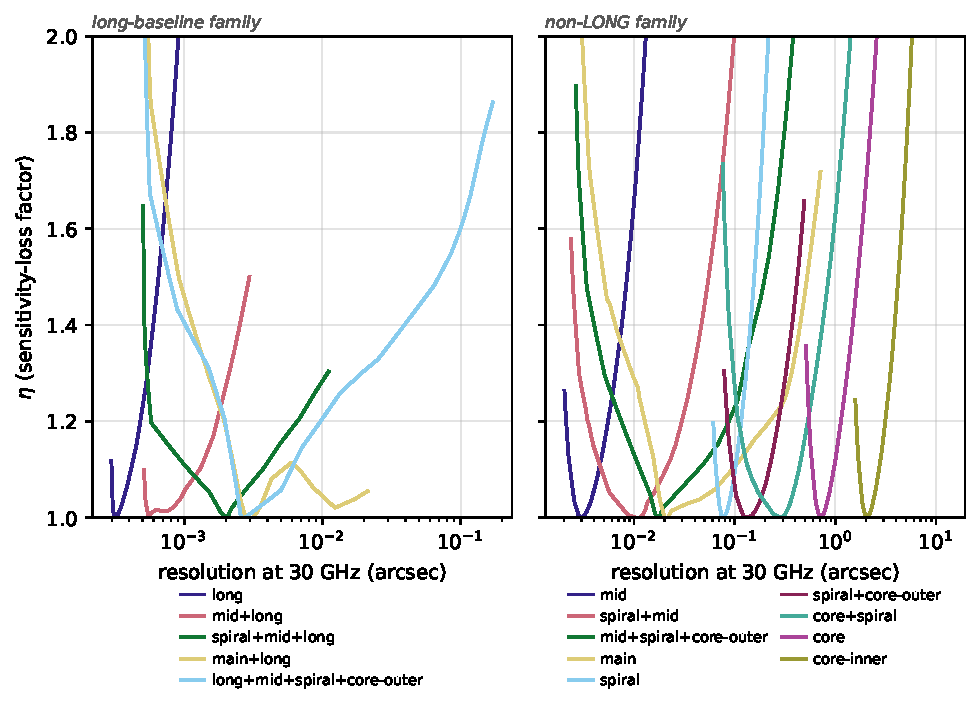
\includegraphics[width=\linewidth]{figs/taperability.pdf}
\caption{Point-source (taperability) envelopes at 30 GHz for the fourteen
offered Rev F subarrays: minimum $\eta$ versus achievable geometric-mean
beam, ignoring PSF shape.  Left: the compact/core family; right: the
long-baseline family (the panels intentionally do not share an x-axis).
Curves are the engine's interpolated envelopes over the measured
(robust, taper) lattice --- the same code path the selector uses --- clipped
at each heterogeneous subarray's beam cap and at the report's $\eta \le 5$
display trim; gaps are unmeasured stretches, not interpolation.}
\label{fig:taperability}
\end{figure}

\begin{figure}[tb]
\centering
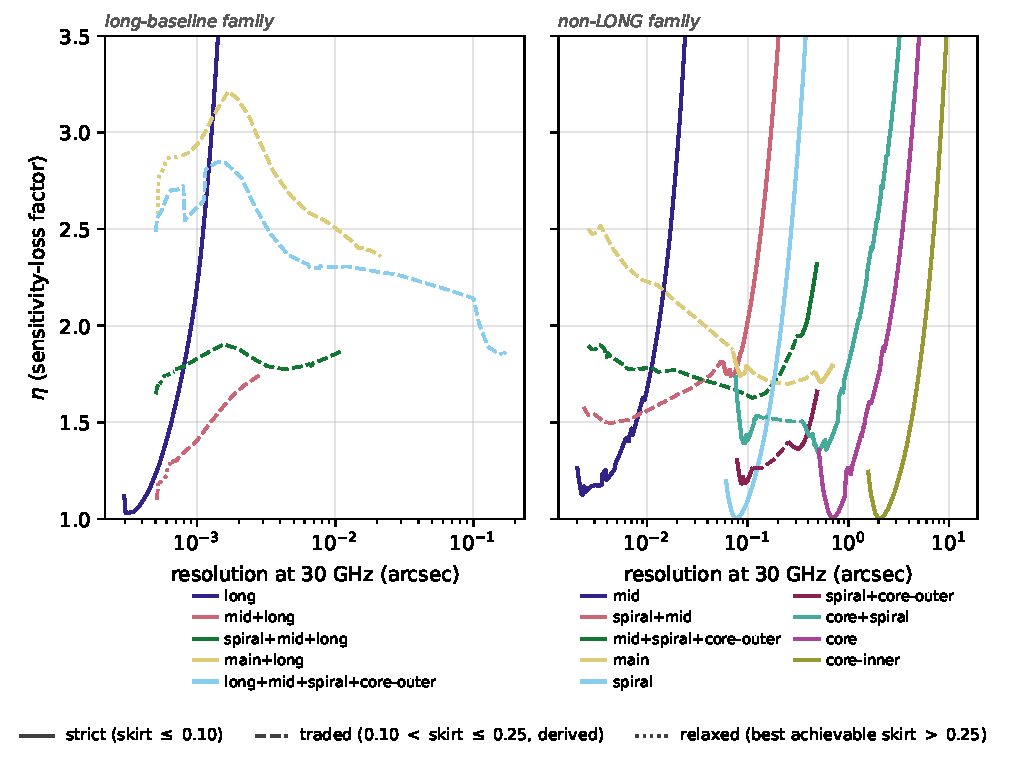
\includegraphics[width=\linewidth]{figs/imaging.pdf}
\caption{Imaging (sculptability) envelopes for the same subarrays under the
default threshold policy with $s_{\max}=0.10$ (panels as in
Fig.~\ref{fig:taperability}).  Solid: strict ($s \le 0.10$ achieved).
Dashed: relaxed points whose best achievable skirt is $\le 0.25$ (the
retired trade cap, kept here purely as a readability bucket).  Dotted:
relaxed points whose best achievable skirt exceeds $0.25$, concentrated near
the finest resolutions of the long-containing composites.  Five of those
composites (mid+long, spiral+mid+long, main+long, mid+spiral+core-outer,
long+mid+spiral+core-outer) never reach the strict threshold anywhere in
their offered range.}
\label{fig:imaging}
\end{figure}

\section{Curve engine: query time}
\label{sec:engine}

The query engine uses the same interpolation code for the selector and for the
HTML report.  Samples are grouped by lattice row, where a row is one
weighting/robust value and taper varies.  Within each accepted adjacent
segment the engine interpolates $\ln \eta$, skirt $s$, and $\ln T$ linearly
in $\ln \theta$.  Column segments do the same along the robust direction at
fixed taper between lattice-adjacent Briggs rows.  Four lattice-adjacent
corner points define a bilinear cell ($\ln\theta$, $\ln\eta$, and $s$
bilinear in normalized cell coordinates); the constrained optimum along a
resolution locus is enumerated analytically.  A cell forms only where all
four edges are free of intervening measured points, so a cell edge
coincides exactly with a row or column segment and never undercuts a more
accurate one-dimensional fit.  The cell construction was validated against
a brute-force two-dimensional oracle on the real Rev F table.  Segment
gates are conservative: segments connect only taper-adjacent samples with
lattice-like taper and resolution steps, exact duplicates are dropped,
robust $-0.0$ is canonicalized to $0.0$, and there is no extrapolation
beyond a row endpoint.

For a request with fractional beam margin $m$, the engine works over the
interval $[\theta(1-m),\theta(1+m)]$ at the 30 GHz reference scale,
intersected with the subarray's beam cap.  The minimum is exact for the
piecewise model.  The candidates are measured points in the interval,
interval endpoints on covered segments, threshold crossings at
$s=s_{\max}$, and the analytic critical points of the bilinear cell
interiors.  The retired trade mode adds the trade-cap crossings and
penalized-branch stationary points, all available in closed form for the
piecewise-log-linear model.

For imaging, the default policy (\emph{threshold} mode, adopted 8 July 2026)
treats the requested resolution as the hard requirement and the skirt as a
quality target.  If any candidate in the interval meets $s \le s_{\max}$
($0.10$ by default), the engine returns the minimum-$\eta$ candidate among
them and labels it strict.  Otherwise it returns the candidate with the
best achievable skirt in the interval, ties broken by $\eta$, flagged
relaxed with that best skirt reported.  No $\eta$ or skirt ceiling is
imposed: the cost is reported and the caller judges.  A hard-threshold variant returns no answer
instead of relaxing (used by the Memo 121 replays of \S\ref{sec:validation}).
The earlier primary objective, the one-for-one eta-skirt trade
\begin{equation}
  J(\theta,p) = \eta(\theta,p) + \max[0,\,s(\theta,p)-s_{\max}],
  \qquad s(\theta,p)\le s_{\max}+0.15 ,
\end{equation}
with $s_{\max}=0.10$ (so the trade extended to a skirt of 0.25), is retired
but retained as a diagnostic/comparison mode; the $0.25$ trade cap survives
in this memo only as a readability bucket in
Figure~\ref{fig:imaging}.

This shared engine replaced a hard per-window sample minimum.  The old rule
converted lattice quantization into isolated pop-ups and drop-outs: a cheap
family could have a hole just wider than the beam margin, or a skirt threshold
could slice between two robust rows.  The internal curve-anomaly post-mortem
\cite{postmortem} documents those mechanisms and motivated the single engine
now used by both the selector and the report.

\begin{figure}[tb]
\centering
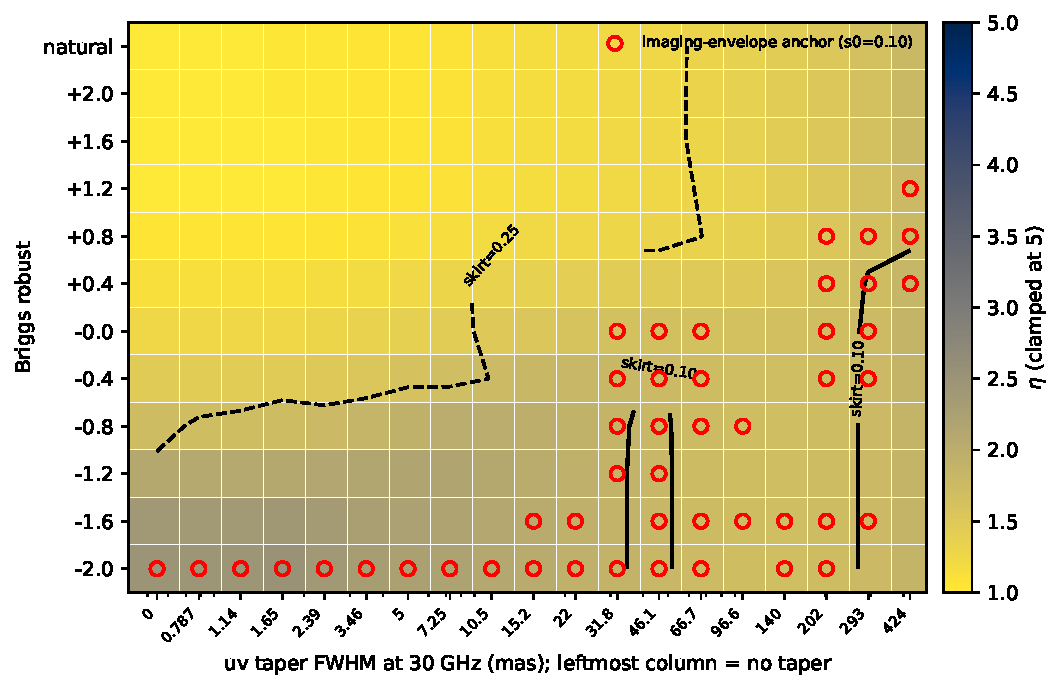
\includegraphics[width=0.95\linewidth]{figs/heatmap.pdf}
\caption{The measured robust--taper lattice for the main subarray, colored
by $\eta$ (clamped at 5).  The untapered column and the natural-weighting
row appear as labeled sentinel bands on the otherwise log-scaled taper axis.
Black contours mark skirt $=0.10$ (solid) and $0.25$ (dashed); their
blockiness is lattice quantization, not a smoothing artifact.  Red circles
mark the lattice cells that anchor the default $s_{\max}=0.10$ imaging
curve.  This lattice is essentially complete: of its 259 sampled points,
255 have status \texttt{ok} and 4 are beam-capped.}
\label{fig:heatmap}
\end{figure}

\section{Selection and ranking}

For each subarray, the selector scales the reference curve to the requested
frequency, evaluates whether the beam can be achieved within the requested
margin, and checks whether the subarray LAS exceeds any requested LAS.  Imaging
requests use the skirt engine above; point-source requests ignore skirt.  A
candidate can therefore be infeasible for three reasons: no beam is
available within the margin, its LAS is too small, or hard-threshold mode
is active and no strict point exists.  Traded and relaxed skirt cases remain
feasible but carry warnings.

The ranking layer is deliberately pluggable.  Built-in choices are minimum
antenna-hours and minimum integration time.  If no sensitivity goal is given,
the same ordering is approximated by radiometer scalings,
$t \propto \eta^2/[N(N-1)]$ and $N t \propto \eta^2/(N-1)$.  Valid requests
are assumed to have positive frequency, resolution, sensitivity, and LAS, with
$0\le m<1$ for the beam margin and physically meaningful skirt thresholds.

Sensitivity calculations use the Memo 96 calculator only for the natural-rms
anchor \cite{memo96}.  The calculator's internal $\eta_w(\theta)$ is a
placeholder and is not used.  Instead, the wrapper calls the calculator at
native resolution, where its internal factor is unity, and applies the curve
engine's $\eta$:
\begin{equation}
  \sigma_{\rm req} = \eta_{\rm curve}\,\sigma_{\rm nat}.
\end{equation}
Flux-density goals are handled directly.  Brightness-temperature goals are
converted to Jy per beam using the requested beam and frequency.  The
calculator lacks a core+mid entry, so core+mid is donor-rescaled from main by
the exact 18-m thermal-noise factor
\[
\sqrt{N_{\rm main}(N_{\rm main}-1)\,/\,
      [N_{\rm core+mid}(N_{\rm core+mid}-1)]}\,.
\]
The confusion term is negligible at these native resolutions in the current
calculator path.  The same $N(N-1)$ rescale corrects any campaign whose
antenna counts differ from the calculator's tables (Rev C.01's do; Rev F's
and Rev D's match, so the factor is exactly one there).

\section{Validation}
\label{sec:validation}

Memo 121 replays run in hard-threshold mode to verify that known EOP-style
assignments can be reproduced.  This is a validation of interpretation and
units, not a claim that the bootstrap Memo 121 curves are the final Rev F
performance table.

Independent Stroh cross-checks validate several pieces and leave one open
issue \cite{stroh}.  His tabulation stored a scalar beam as
$\sqrt{b_{\rm maj}^2+b_{\rm min}^2}$ despite comments describing a geometric
mean; after dividing by $\sqrt{2}$, core, spiral, and mid native beams agree
with the Rev F pipeline to within about one percent.  Core and mid eta curves
agree at the few-percent level.  The spiral eta curve disagrees substantially
near its coarse end, and the raw Stroh tabulation needed to resolve that
discrepancy is not in the delivered package.  This is therefore a bounded
cross-check, not a complete external validation.

The engine also has envelope-consistency and spike-census QA.  Named
post-mortem anomalies are regression-tested on the real Rev F curve table, and
the report uses the same engine as the selector to avoid policy divergence.
Stair-step behavior from robust-direction quantization was subsequently
removed by the column-segment densification; residual curve steps on the real
data are below $\sim$0.16 in $\eta$ away from the $\eta$-cap fringe and are
regression-tested.

\section{Limitations and future work}
\label{sec:limitations}

The main algorithmic limitation is the bilinear model within lattice cells:
the residual error is bounded by the true surfaces' within-cell curvature
relative to a bilinear fit and shrinks as the lattice is filled (held-out
recovery on the Rev F table shows median interpolation errors of
0.2--2.7\% in $\eta$ in the operating range).  The adaptive retrofit
(\S\ref{sec:refinement}) has run one wave over all four completed
campaigns; several Rev F and Rev D track maps stopped at the per-map audit
cap, so further waves to full certification remain queued.  Targeted
contour sampling near the $s=s_{\max}$ surface is the next refinement if
needed.

The physical limitations are separate.  Current curves use one noise
realization, so noise-floor sensitivity of $\eta$ is not fully quantified.
Frequency scaling assumes $\eta$ invariance and ignores fractional-bandwidth uv
filling changes.  The Memo 121 fixed-FOV, single-pointing convention is assumed;
PLAN section 12 identifies mosaics, field-of-view dependence, and spectral-line
uv filling as open use cases \cite{plan}.  The Memo 67 LAS coefficient is
applied uniformly to all 18-m subarrays and is assumed independent of robust
and taper.  SBA remains deferred (6-m dishes, no taper support in the
sensitivity calculator).  Long is now included via the 178 m
spurious-shorts uv filter (\S\ref{sec:curvegen}), with one residual caveat:
main+long is unfiltered, so its raw $b_{\min}$ makes its quoted LAS likely
optimistic.  The sensitivity calculator also recenters continuum requests to
receiver-band midpoints internally, while the curve/LAS scaling currently uses
the requested frequency.  The snapshot campaign tables are collected but not
released: their sparse instantaneous uv coverage produces genuine
resolution discontinuities (certified by the adaptive sampler,
\S\ref{sec:refinement}) that the release conventions do not yet present
well.  The Rev C.01 track table is staged but not yet measured at this
writing.  All quantitative results here are Rev F four-hour-track values.

\appendix
\section{Data products}

\begin{table}[tb]
\centering
\small
\caption{Primary data products used by the memo and selector.}
\label{tab:products}
\begin{tabular}{@{}p{0.34\linewidth}p{0.14\linewidth}p{0.44\linewidth}@{}}
\toprule
Product & Role & Notes \\
\midrule
\texttt{curvegen/results*/*.csv} &
Sweep measurements &
One row per measured, skipped, capped, or failed lattice point; non-default
campaigns use \texttt{results-} \texttt{<rev>\_<mode>/}. \\
\texttt{sa\_select/data/} \texttt{config\_registry.csv} &
Campaign registry &
Routes each (revision, simulation-mode) pair to its metadata and curve CSVs. \\
\texttt{sa\_select/data/} \texttt{revf\_curves.csv} &
Query samples &
Collected status-\texttt{ok} Rev F rows, with $\eta$ normalized to natural;
other campaigns collect to their registered
\texttt{<rev>\_<mode>\_curves.csv}. \\
\texttt{sa\_select/data/} \texttt{subarrays*.csv} &
Subarray metadata &
Names, components, antenna counts, physical baselines, LAS coefficient, and
measured beam caps; one file per registered campaign. \\
\texttt{curvegen/reports/*.html} &
QA/report &
Regenerable local reports using the same shared envelope engine. \\
\bottomrule
\end{tabular}
\end{table}

\begin{table}[tb]
\centering
\small
\caption{\texttt{revf\_curves.csv} schema.}
\label{tab:schema}
\begin{tabular}{@{}p{0.32\linewidth}p{0.12\linewidth}p{0.48\linewidth}@{}}
\toprule
Column & Unit & Meaning \\
\midrule
\texttt{subarray} & -- & Canonical subarray name. \\
\texttt{resolution\_arcsec\_30ghz} & arcsec & Geometric-mean FWHM at 30 GHz. \\
\texttt{eta} & -- & Dirty-rms ratio to untapered natural weighting. \\
\texttt{skirt} & peak fraction & PSF radial mean at one fitted FWHM. \\
\texttt{weighting} & -- & \texttt{natural} or \texttt{briggs}. \\
\texttt{robust} & -- & Briggs robust value; blank for natural weighting. \\
\texttt{taper\_arcsec\_30ghz} & arcsec & Outer uv taper FWHM on the sky at 30 GHz. \\
\texttt{freq\_orig\_ghz} & GHz & Simulation/reference frequency, currently 30.0. \\
\texttt{source} & -- & Provenance string linking back to sweep point. \\
\texttt{note} & -- & Free-form caveat, including interpolated-anchor notes. \\
\texttt{sample\_status} & -- & Collection status; only \texttt{ok} rows enter the engine. \\
\bottomrule
\end{tabular}
\end{table}

\section{How to run the campaigns and reports}
\label{sec:runbook}

This appendix is the short form.  \texttt{RUN\_CAMPAIGNS.md} in the
repository is the full run sheet, with monitoring and failure recovery.

The environment is TACC Stampede3.  Use the CASA~6 Python wrapper
\texttt{casapy}
(\texttt{/work2/.../casaenv/bin/casapy}).  Keep measurement sets on
\texttt{\$WORK} (\texttt{NGVLA\_MS\_BASE}) and \texttt{tclean} scratch on
\texttt{\$SCRATCH} (\texttt{NGVLA\_SCRATCH}).  Submit jobs from a login
node.

To run one campaign, first submit the three-stage chain.  After its collect
stage finishes, submit the PSF-cut backfill for that campaign's combo
index:
\begin{verbatim}
bash curvegen/submit_campaign.sh <rev> <sim_mode> --time 47:00:00
sbatch --array=<combo> --dependency=afterok:<collect_id> \
       curvegen/backfill_psf.sbatch
\end{verbatim}
Combo indices are 0 =\,revF/track, 1 =\,revF/snapshot, 2 =\,revD/track,
3 =\,revD/snapshot, 4 =\,revC/track.  Every stage is resumable: re-run the
same command and only missing work executes.  \texttt{--prep-only} stops
after the quality-assurance gate.

To improve converged coverage on an existing campaign, run the adaptive
retrofit (one array task per combo, each ending with its own collect,
report, and PSF export):
\begin{verbatim}
sbatch --array=<combos> curvegen/adaptive_retrofit.sbatch
\end{verbatim}

To rebuild the reports locally (no Slurm needed):
\begin{verbatim}
cd curvegen
casapy make_report.py --combined reports/ngvla-curves.html
casapy make_report.py --combined --release \
       reports/ngvla-curves-release.html
\end{verbatim}
The first is the internal all-campaigns page.  The second is the released
page: the three released campaigns only, with the imaging sections of the
point-source-only campaigns marked ``Omitted / intentionally blank''.

To run the test suite (from the repository root):
\begin{verbatim}
casapy -m unittest discover -s tests -t .
\end{verbatim}

\section{The Python calculator interface}
\label{sec:pyinterface}

The calculator is the \texttt{sa\_select} package.  It needs numpy at query
time and scipy only for sensitivity goals; it does not need CASA.

From Python, build a request and rank the subarrays:
\begin{verbatim}
from sa_select import (ObservingRequest, select_subarrays,
                       CurveLibrary)

request = ObservingRequest(
    resolution=0.005,      # arcsec
    frequency=30.0,        # GHz
    sensitivity=1e-6,      # Jy/beam (optional)
    las=1.0,               # arcsec (optional)
    imaging=True,          # False = point-source
    beam_margin=0.05)      # fractional beam tolerance

library = CurveLibrary.for_config("revF", "track")
result = select_subarrays(request, library=library)
print(result.table())      # or result.to_rows() for dicts
best = result.best         # top-ranked feasible Candidate
\end{verbatim}
Each feasible \texttt{Candidate} carries the achieved beam, $\eta$, the
\texttt{tclean} weighting (\texttt{weighting}, \texttt{robust},
\texttt{taper}), the skirt, the LAS, the integration time and antenna-hours
(when a sensitivity goal was given), and any warnings.  Infeasible
subarrays are kept with their exclusion reasons.  The ranking heuristic is
pluggable: pass \texttt{heuristic=} a built-in name
(\texttt{antenna\_hours}, \texttt{integration\_time}) or any callable.

The same engine runs from the command line:
\begin{verbatim}
python3 -m sa_select --resolution 0.005 --frequency 30 \
    --sensitivity 1e-6 --point-source --rev revD
\end{verbatim}
\texttt{--rev}/\texttt{--sim-mode} select any registered campaign.  An
imaging query against a point-source-only released campaign (Rev D track,
Rev C.01 track) prints a warning and still runs.

Batch mode reproduces an EOP-style case list: give a CSV with one request
per row (columns \texttt{case, resolution, frequency, sensitivity,
sensitivity\_unit, las, imaging, beam\_margin, skirt\_threshold, optimize,
delta\_v}; empty cells fall back to the command-line flags) and get one CSV
row per case per ranked candidate:
\begin{verbatim}
python3 -m sa_select --batch cases.csv --top 3
\end{verbatim}

Stroh-format inputs are supported (\texttt{sa\_select/stroh.py}).
\texttt{--stroh subarray\_data.json} queries M.~Stroh's delivered curve
package directly: the loader converts his $\sqrt{2}$ quadrature beam
convention to geometric-mean FWHM and evaluates his splines
\cite{stroh}.  Those curves are point-source only, and his delivery does
not record which (robust, taper) achieves each point, so the reported
taper is a placeholder and every result carries a warning that says so.
The module also reads his per-subarray CASA \texttt{.cfg} files into
subarray metadata (physical baselines, with an optional
spurious-short-baseline cut).

\begin{thebibliography}{9}

\bibitem{memo55}
\ngvla\ Memo 55, taperability and weighting efficiency.

\bibitem{memo65}
\ngvla\ Memo 65, PSF sculpting metric and robust/taper grids.

\bibitem{memo67}
\ngvla\ Memo 67, largest angular scale simulations and LAS coefficients.

\bibitem{memo72}
\ngvla\ Memo 72, taperability and sensitivity-loss conventions.

\bibitem{memo76}
\ngvla\ Memo 76, subarray-selection lookup table context.

\bibitem{memo96}
\ngvla\ Memo 96, \ngvla\ sensitivity calculator.

\bibitem{memo121}
\ngvla\ Memo 121, skirt threshold, sculptability, and EOP assignments.

\bibitem{plan}
\texttt{PLAN.md}, implementation plan and current open questions, especially
section 12.

\bibitem{postmortem}
\texttt{curve\_anomaly\_postmortem.md}, internal post-mortem on quantization
artifacts and shared-engine requirements.

\bibitem{stroh}
\texttt{mstroh\_comparison.md}, internal comparison with Michael Stroh's
taper-simulation package.

\end{thebibliography}

\end{document}
